
\chapter{Reperimento delle Informazioni per Ricerche Testuali}


Parlando di “Reperimento delle Informazioni” (in inglese \textit{Information Retrieval}, abbreviato IR) si fa riferimento a problemi ed esigenze che non caratterizzano la sola età moderna: l’essere umano ha da sempre avuto la necessità di reperire informazioni in maniera semplice ed efficace. Fino a qualche decennio fa, l’unico modo per poter cercare e ritrovare informazioni ben precise, contenute all’interno di una base documentale, consisteva nel suddividere e catalogare le fonti a propria disposizione, quanto più precisamente possibile, in biblioteche e archivi.

\vspace{1em}

L’avvento dei computer ha aperto nuove opportunità. Se precedentemente era impensabile poter cercare una specifica frase o immagine all’interno di una collezione di libri, ciò è stato reso possibile grazie al trattamento dell’informazione in formato digitale. La rappresentazione di una crescente mole di documenti in digitale e la necessità di reperire velocemente informazioni in grado di soddisfare le esigenze informative dell’utente sono i motivi che hanno contribuito alla nascita dell’Information Retrieval (IR), che vede la luce nei primi anni ’60 e trova il suo massimo punto di espansione dopo gli anni ’90, con l’avvento del World Wide Web.

\vspace{1em}

L’\textbf{Information Retrieval} è la disciplina informatica che si occupa della rappresentazione e dell’organizzazione di ingenti quantità di risorse digitali, al fine di consentire il reperimento di informazioni che si rivelino utili a soddisfare specifiche necessità informative espresse dall’utente mediante la formulazione di una \textit{query}. Il risultato principale degli studi e della ricerca nel campo dell’IR sono i \textbf{motori di ricerca}, \textit{Information Retrieval System} (abbreviato in IRS) che svolgono il ruolo di intermediari fra sorgenti dei dati e utente finale. In questa tesi si sono considerati motori di ricerca che gestiscono esclusivamente collezioni di testi.
\pagebreak




\section{Struttura di un Information Retrieval System}

Un sistema di reperimento delle informazioni è costituito da molteplici componenti che cooperano per

\begin{itemize}
\item rappresentare formalmente i documenti che costituiscono l’archivio dei dati
\item formalizzare le esigenze informative dell’utente, espresse attraverso la formulazione di una query
\item confrontare query e documenti
\item presentare all’utente i documenti che vengono stimati rilevanti rispetto alla query
\end{itemize}

\begin{figure}[H]
	\centering
	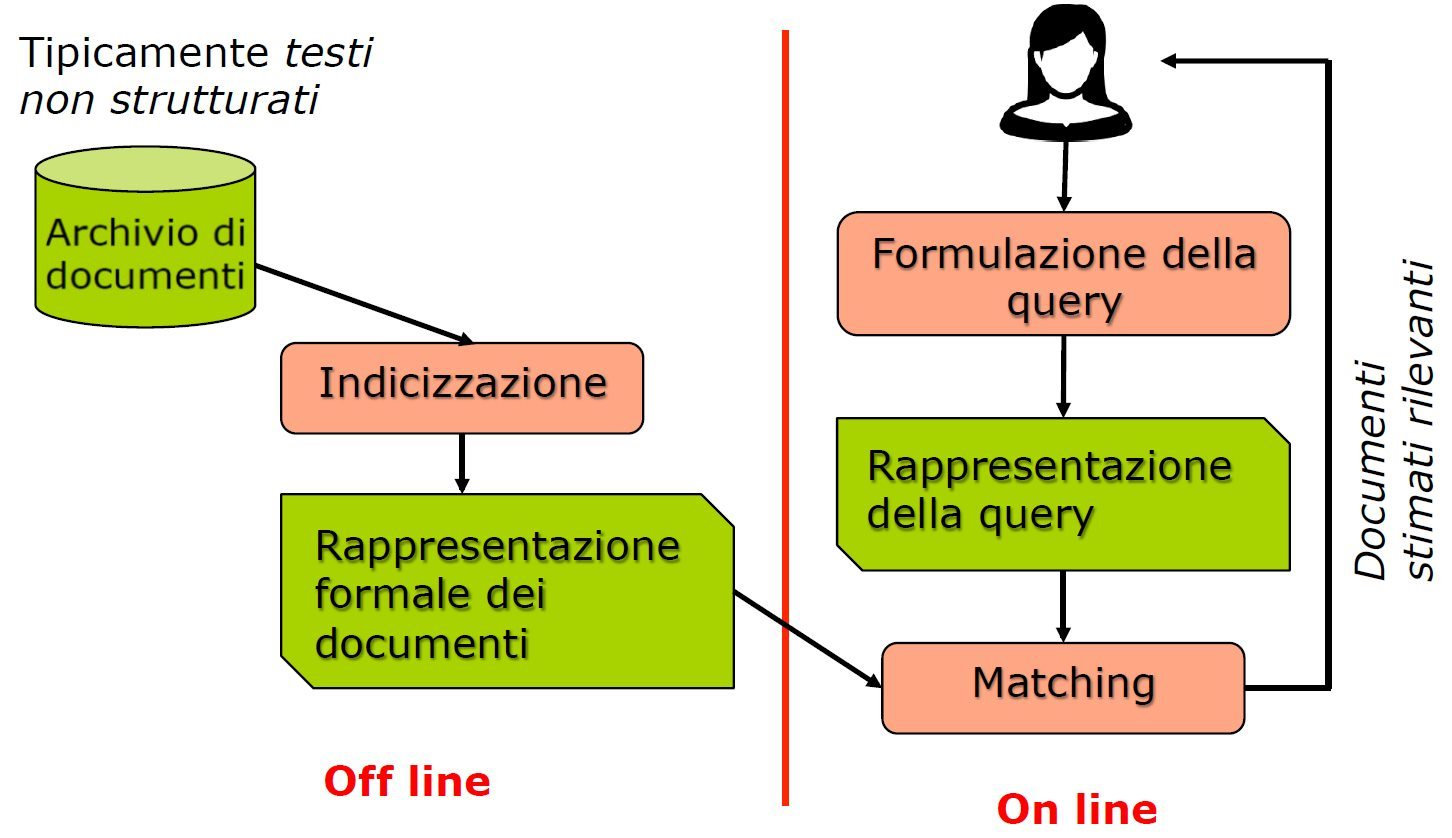
\includegraphics[scale=0.7]{../images/01_1_struttura_IRS}
	\caption[Struttura di un IRS]{Struttura di un IRS}
	\label{fig:strutturaIRS}
\end{figure}

L’obiettivo principale dell'IRS consiste nel reperire, a seguito di una query, tutti i documenti rilevanti per l’utente, minimizzando al contempo il reperimento di documenti non rilevanti. Il concetto di \textbf{rilevanza}, difficile sia da modellare che da valutare, esprime l’utilità di un documento nel soddisfare una specifica esigenza informativa e costituisce uno degli elementi chiave attorno al quale si sviluppa un IRS.

Un sistema per il reperimento delle informazioni è basato su un \textbf{modello matematico} che consente di produrre una rappresentazione formale del problema e di definire opportune metodologie di confronto, in grado di stimare la rilevanza di un documento rispetto ad una query. Si rivela difficile valutare la correttezza del risultato prodotto dal confronto, poiché influenzato da numerosi fattori di incertezza e soggettività.

\vspace{1em}

Seppur l’unica parte visibile di un motore di ricerca sia costituita dall’interfaccia che consente all’utente di formulare delle query e consultarne i risultati, la ricerca è frutto di una catena di operazioni complessa, approfondita gradualmente nel corso della tesi fino allo sviluppo di un motore di ricerca vero e proprio.
\pagebreak




\section{Indicizzazione del testo}

Un sistema di reperimento delle informazioni opera con archivi costituiti come agglomerato di documenti che provengono da sorgenti di diversa natura. Il primo compito del sistema consiste nell’elaborazione di ciascun documento per ricavarne il contenuto informativo, affinché possa essere catalogato e memorizzato nella maniera opportuna.

Questo processo è detto \textbf{indicizzazione} e consiste nell’estrazione, da un documento, di opportuni “descrittori” in grado di rappresentarne formalmente ed esaustivamente il contenuto. Il risultato di questa elaborazione sono gli \textbf{indici}, strutture dati che costituiscono l’elemento base della rappresentazione formale di un archivio documentale e consentono di reperire informazioni in maniera molto rapida.

\vspace{1em}
Gli indici adibiti alla rappresentazione di archivi testuali devono essere:
\begin{itemize}
\item \textbf{esaustivi}, cioè rappresentare tutti gli argomenti trattati nel testo;
\item \textbf{specifici}, cioè in grado di discriminare il contenuto di due documenti diversi.
\end{itemize}

Fra le possibili soluzioni per l’analisi e l’indicizzazione del testo, una delle tecniche principali per la sua rappresentazione consiste nell’indicizzarne il contenuto per singoli \textbf{termini}. Ciò consiste in un processo di trasformazione del testo originario in un flusso di \textit{token}, ovvero sequenze di caratteri (come le parole), che vengono successivamente elaborati per ricavare i termini da inserire nell’indice. I termini indice sono l’elemento base di un sistema di reperimento delle informazioni, in quanto sia la ricerca che le strutture di memorizzazione sono pensate per operare su insiemi di termini.

L’indicizzazione si rivela di fondamentale importanza, poiché è durante questa fase che un IRS decide cosa sia opportuno memorizzare, cosa invece scartare ed eventualmente come far sì che determinate informazioni appaiano più “importanti” di altre, cioè più adatte a descrivere efficacemente il contenuto di un documento. A tale scopo, è possibile catalogare gli elementi estratti da un documento per differenziare il trattamento che sarà riservato a ciascuno di essi. Ad esempio, è possibile determinare in che modo sia necessario elaborare e memorizzare l’\textit{oggetto} piuttosto che il \textit{corpo} o il \textit{mittente} di una email.


\subsection{Estrazione dei termini}

L’analisi del testo, che consente di ricavarne i termini da indicizzare, è un processo meticoloso che si compone di molteplici passaggi, i quali costituiscono il primo passo per la rappresentazione formale dei documenti. Un IRS non è tenuto ad implementare l’intera catena di analisi del testo, ma è fondamentale che tale analisi sia effettuata in maniera compatibile anche durante la fase di interrogazione, affinché il meccanismo di confronto fra documenti e query sia in grado di produrre risultati attendibili.


\subsubsection{Suddivisione in Token}

Tutto comincia con la suddivisione del flusso di caratteri del testo originale in \textit{token}, ricavati dalla separazione tramite spazi o segni di punteggiatura. In linea di massima, ogni parola è un \textit{token}, ma può capitare che per la separazione dei termini vengano sfruttati per esempio anche numeri (\textit{peer2peer}), caratteri speciali (\textit{wi-fi}) o maiuscole (\textit{WiFi}).

\begin{figure}[H]
	\centering
	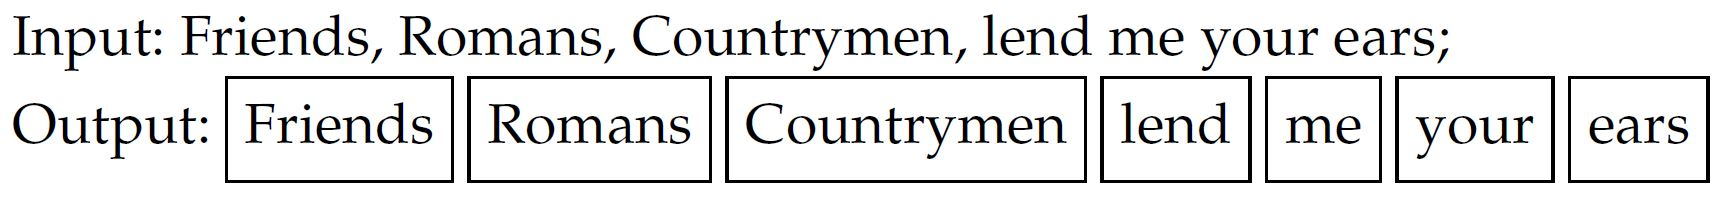
\includegraphics[scale=0.33]{../images/01_2_esempio_token}
	\caption[Esempio di suddivisione in \textit{token}]{Esempio di suddivisione in \textit{token}}
	\label{fig:tokenexample}
\end{figure}

Ogni \textit{token} viene successivamente “normalizzato” tramite l’applicazione di un insieme di regole scelte arbitrariamente. Ad esempio, spesso accade che le lettere maiuscole vengano sostituite con le corrispondenti minuscole e che la medesima sorte sia riservata alle lettere accentate, rimpiazzate dalla propria forma base (\textit{è} diventa \textit{e}, \textit{Ü} diventa \textit{u}).


\subsubsection{Rimozione delle Stop Word}

Ogni lingua è caratterizzata da un insieme di parole che sono molto frequenti all’interno di un testo: articoli, preposizioni, pronomi, avverbi, verbi ausiliari, … Considerata l’elevata frequenza con la quale vengono utilizzate, esse risultano poco adatte a descrivere il contenuto di un documento e influiscono negativamente sulla dimensione degli indici, motivi per cui è consuetudine ignorarle o rimuoverle durante il processo di indicizzazione. Queste prendono il nome di \textit{stop word} e sono caratteristiche di ciascuna lingua.


\subsubsection{Stemming}
Anche nel caso dello \textit{stemming} ci si trova di fronte ad un caso di analisi linguistica.\newline
Consiste nella “contrazione” di alcune parole alla loro forma base o alla radice di appartenenza, operazione che può essere effettuata nel caso ci si trovi ad esempio in presenza di plurali, verbi o parole che derivano da altre. Come la rimozione delle \textit{stop word}, non è una fase obbligatoria dell’analisi testuale ma porta dei benefici sia in termini di dimensione degli indici che dal punto di vista delle interrogazioni, che grazie allo \textit{stemming} possono godere di una maggiore flessibilità (ad esempio, facendo sì che cercare \textit{studente} o \textit{studenti} produca i medesimi risultati).

Per essere precisi, sarebbe opportuno specificare che lo \textit{stemming}, seppur dipendente dalla lingua, consiste semplicemente nell’applicazione di alcuni algoritmi che troncano le parole secondo determinate regole prestabilite. Se si vuole ottenere un risultato più accurato e ridurre davvero ciascuna parola alla propria forma canonica (lemma) - ad esempio, in italiano, i verbi al proprio infinito - si dovrebbe parlare di \textbf{lemmatizzazione}, un’operazione più complessa che sfrutta opportuni dizionari linguistici.


\subsubsection{Espansione dei Termini}

Spesso accade che, sia in fase di indicizzazione che durante un’interrogazione, alcuni termini possano rivelarsi troppo specifici o, al contrario, troppo generici. Ne è un esempio il caso in cui cercando la parola \textit{animale} un utente si aspetta che vengano reperiti anche tutti i documenti in cui compaiono le parole \textit{cane} e \textit{labrador}. Inoltre, si verifica spesso che una stessa parola possa assumere significati diversi a seconda del contesto all’interno del quale viene utilizzata. Per questi motivi è efficace poter definire delle correlazioni fra alcuni termini, assegnandovi significati e sinonimi specifici del contesto di appartenenza. Ciò è possibile attraverso l’utilizzo di appositi dizionari e tesauri (tematici o linguistici) che consentano di effettuare l’espansione di ciascun termine con altri ad esso correlati. Il vantaggio consiste nell’esecuzione di ricerche più utili per l’utente.

Questa è probabilmente la fase più complessa dell’analisi testuale poiché altamente dipendente sia dalla lingua che dal contesto applicativo. Un’opportuna implementazione richiede l’utilizzo di risorse costruite \textit{ad hoc} per la realtà all’interno del quale si inserisce il motore di ricerca.



\subsection{Pesatura dei termini}
\label{sec:termsweight}

Ottenuta la lista dei termini che compongono la base di dati testuale, è fondamentale decidere il criterio secondo il quale l’occorrenza di un termine in un certo documento influisca sui risultati della ricerca in atto da parte dell’utente. È chiaro che non tutte le parole di un documento siano ugualmente utili a descriverne il contenuto informativo, pertanto si rivela fondamentale la possibilità di assegnare a ciascun termine un \textbf{peso}, che esprima l’importanza del termine stesso come descrittore del documento.

\vspace{1em}

Una pesatura dei termini di tipo binario (\texttt{1} se il termine compare in un certo documento, \texttt{0} se non compare) non è sufficiente per ottenere dei risultati di ricerca abbastanza significativi. Per ogni termine è estremamente importante valutare anche quale sia la \textbf{frequenza} con cui appare sia all’interno di uno specifico documento, sia nell’intera collezione. Per questo motivo si è sviluppato il modello di pesatura dei termini conosciuto come \textit{TF*IDF}. Secondo quest’ultimo, il peso \(w_{ij}\) di un certo termine \(t_{j}\) nel documento \(d_{j}\) prende il nome di \textbf{significatività}, che può essere calcolata con la seguente funzione matematica:

\[ w_{ij} = f_{ij} \times log\frac{N}{d_{fi}} \]

Il primo fattore \(f_{ij}\) rappresenta la frequenza (il numero di occorrenze) del termine  \(t_{i}\) nel documento \(d_{j}\). \newline
Il secondo fattore è detto \textit{inverse document frequency (IDF)} ed è tanto più alto quanto minore è il numero di documenti in cui il termine \(t_{i}\) compare (\(N\) è il numero totale di documenti nella collezione e \(d_{fi}\) è il numero di documenti che contengono il termine \(t_{i}\)).

Poiché la frequenza di un termine in un documento cresce naturalmente con la lunghezza del documento stesso, è opportuno che il parametro \(f_{ij}\) venga normalizzato come segue:

\[ w_{ij} = \frac{tf_{i}}{\max tf_{j}} \times log\frac{N}{d_{fi}} \]

\vspace{1em}
Dividendo la \textit{frequenza assoluta} \(tf_{ij}\) (del termine \(t_{i}\) nel documento \(d_{j}\)) per la \textit{frequenza massima} di tutti i termini in \(d_{j}\) si ottiene come primo fattore la \textit{frequenza relativa (TF)} del termine \(t_{i}\) nel documento \(d_{j}\).
Così facendo, si è in grado di pesare ogni termine sulla base della frequenza cui compare all’interno dell’intera collezione e di ogni specifico documento, di cui per ognuno se ne considera anche la lunghezza.



\section{Strutture dati per la ricerca: gli indici inversi}

Si è visto che il processo di indicizzazione ha lo scopo di analizzare l’archivio documentale per estrarre gli opportuni descrittori di ciascun documento. Questo processo produce ciò che vengono definiti indici, apposite strutture dati in grado di garantire risposte molto rapide alle richieste dell’utente. Gli indici sono costruiti \textit{offline}, cioè prima che venga messa a disposizione la funzionalità di ricerca, perché la loro costruzione è un processo che può richiedere diverso tempo e risorse.

\vspace{1em}

Di tutte le metodologie atte a memorizzare fisicamente indici \textit{full text} verrà qui presentata solamente quella che sfrutta i cosiddetti \textbf{indici inversi}, molto veloci in termini di reperimento delle informazioni e largamente utilizzati su scala commerciale.

La dicitura “inverso” deriva dall’idea di base che costituisce questo tipo di indici. Si potrebbe ingenuamente pensare di memorizzare, per ogni documento, una lista di termini che vi compaiono, magari all’interno di una matrice statica di natura sparsa. Oltre che uno spreco di spazio, questa è anche una soluzione poco adatta alle nostre esigenze; \textbf{ogni ricerca è di fatto incentrata sui termini} ed in quanto tale è molto più facile reperire i documenti in cui compare un certo termine se la matrice precedentemente accennata viene memorizzata in maniera inversa: \textbf{per ogni termine viene salvata una lista (dinamica) di documenti in cui esso compare}.

In questo modo l’insieme di tutti i termini costituisce il \textbf{dizionario} dell’indice. Ogni termine del dizionario è associato alla propria frequenza globale e possiede un puntatore al \textit{posting file}, che a sua volta contiene la lista di documenti all’interno dei quali il termine compare. Per ogni elemento della \textit{posting list} viene memorizzato l’\textit{identificatore} univoco del documento, la \textit{frequenza} del termine al suo interno e tutte le relative \textit{occorrenze}; per ciascuna occorrenza è possibile memorizzare anche la \textit{posizione} del termine nel documento, per agevolare interrogazioni in cui compaiano operatori di prossimità fra termini.

\vspace{1em}
Questo tipo di memorizzazione consente, in fase di ricerca, di accedere molto velocemente al dizionario e, successivamente, alla \textit{lista di posting} associata al termine trovato nel dizionario. Qualora la query sia composta da termini multipli, ognuno di questi è sottoposto al medesimo trattamento e il risultato finale è costituito da un opportuno \textit{merge} dei risultati parziali.

\begin{figure}[H]
	\centering
	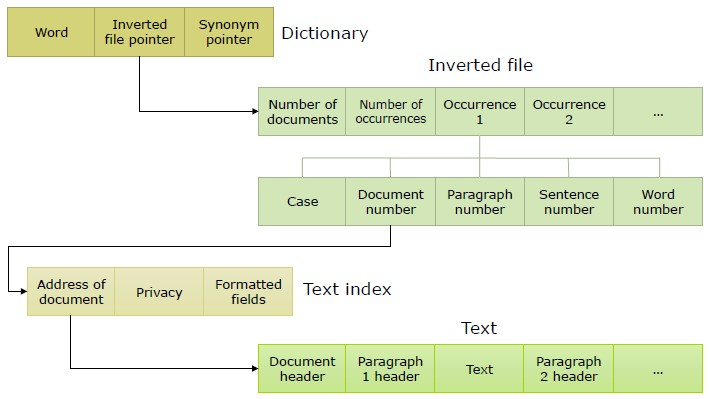
\includegraphics[scale=0.46]{../images/01_3_indice_inverso}
	\caption[Struttura a File Inverted]{Struttura a File Inverted}
	\label{fig:invertedfile}
\end{figure}




\section{Modalità di interrogazione}
\label{sec:mathmodels}

La fase d’interrogazione è l’unica parte di un IRS visibile all’utente, composta da un’interfaccia che gli consenta di esprimere delle \textbf{query}, elaborate dal sistema per produrre risultati coerenti con quanto richiesto. È importante che il linguaggio di interrogazione sia semplice e intuitivo per l’utente, ma abbastanza completo per garantire un certo grado di flessibilità.

Per quanto riguarda l’utilizzo dei motori di ricerca sul Web, una query è mediamente composta da 2-3 parole~\cite{datigoogle} e spesso alla prima ricerca ne seguono altre per raffinare il risultato; molto difficilmente si arriva a sottoporre interrogazioni complesse, che ad esempio si avvalgano di operatori logici\footnote{Alcuni esempi di interrogazioni complesse con Google e Bing:  \url{http://advangle.com/}}.

Approfondendo le modalità con le quali le interrogazioni vengono gestite ed elaborate ci si accorge in maniera evidente che un sistema di Information Retrievial sia in realtà basato su un \textbf{modello matematico}, il quale fornisce innanzitutto una \textbf{descrizione formale dei documenti e delle query}, per consentire in seguito di mettere a confronto i due elementi. Il meccanismo di confronto è detto \textbf{\textit{matching}} e ha lo scopo di \textbf{stimare la rilevanza} di ogni documento rispetto alla query; fornisce pertanto solamente un’approssimazione dell’insieme di documenti che sono davvero rilevanti, producendo un \textbf{risultato incerto}, influenzato negativamente dall’ambiguità del contenuto dei documenti e delle richieste, nonché dalla soggettività di ciascun utente rispetto al concetto stesso di rilevanza.

\begin{figure}[H]
	\centering
	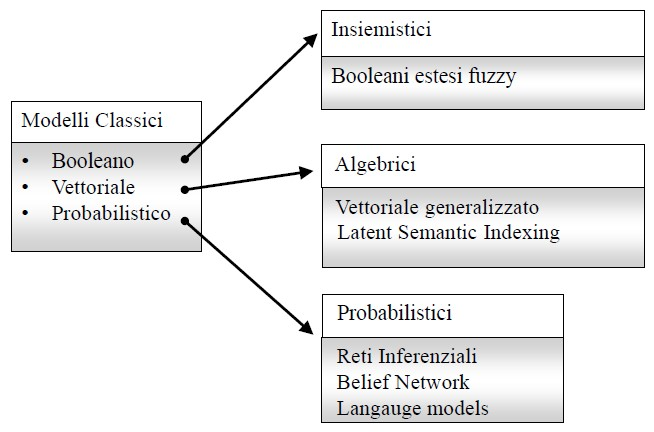
\includegraphics[scale=0.5]{../images/01_4_modelli_matching}
	\caption[Modelli matematici per la rappresentazione di IRS]{Modelli matematici per la rappresentazione di IRS}
	\label{fig:mathmodels}
\end{figure}

I modelli matematici disponibili per la rappresentazione di un IRS sono molteplici e in questa sede vengono brevemente descritti solamente quelli booleano e vettoriale, da cui si sviluppano modelli più complessi e comunemente utilizzati.



\subsection{Modello booleano}

Nel modello booleano la significatività dei termini è rappresentata da pesi binari \(w_{ij}\), pari a \texttt{1} se il termine \(t_{i}\) compare nel documento \(d_{j}\) e pari a \texttt{0} se invece non compare. Il documento \textit{j}-esimo è rappresentato dall’insieme dei termini tale per cui \(w_{ij} = 1\).

Una query è formalmente definita come \textbf{espressione booleana sui termini} e definisce l’insieme di elementi da selezionare tramite l’utilizzo degli operatori logici, che vengono tradotti in operazioni insiemistiche sui documenti: gli operatori \texttt{AND}, \texttt{OR} e \texttt{NOT} corrispondono rispettivamente alle operazioni di intersezione, unione e differenza.

Con questo modello, per ogni termine che compare nella query viene recuperata nell’indice inverso la lista dei documenti associata a tale termine; poi sulle liste dei documenti vengono effettuate le opportune operazioni insiemistiche che danno origine ad un risultato composto dai soli documenti considerati rilevanti.

\vspace{1em}

Nonostante il linguaggio di interrogazione booleano si rilevi particolarmente intuitivo e adatto a modellare sufficientemente le esigenze dell’utente, considerare la rilevanza come proprietà binaria (un documento è rilevante oppure non rilevante) non favorisce ricerche particolarmente utili. Infatti, questo tipo di modellazione ignora completamente la frequenza dei termini all’interno dei documenti e ciò rende impossibile presentare la lista dei risultati in ordine di rilevanza rispetto alla query.



\pagebreak
\subsection{Modello vettoriale}

Il modello vettoriale nasce dall’esigenza di poter modellare la rilevanza come proprietà graduale e permettere l’ordinamento dei risultati di un’interrogazione. Questo modello poggia le propria fondamenta sull’algebra lineare: \textbf{documenti e query sono rappresentati come vettori} all’interno di uno spazio vettoriale \textit{n}-dimensionale, dove \textit{n} corrisponde al numero di termini che appartengono al dizionario degli indici.
Si assume che i termini del dizionario siano linearmente indipendenti fra loro e si rappresenta il termine \textit{i}-esimo come un versore: un vettore di \texttt{zeri} con il peso di valore \texttt{1} alla posizione \textit{i}-esima.
\[ t_{i} = [0, 0, ..., 1, ..., 0, 0] \] % SERVIREBBE METTERE i-1, i, i+1 SOTTO
Analogamente, anche documenti e query sono rappresentati come vettori di pesi, cui ogni posizione è associata all'\textit{i}-esimo termine del dizionario. Ciò consente di effettuare un calcolo di \textbf{similarità} fra il vettore della query e ciascun vettore documento, calcolando di fatto il coseno dell’angolo \(\alpha\) che disegnano i rispettivi vettori.

\begin{figure}[H]
	\centering
	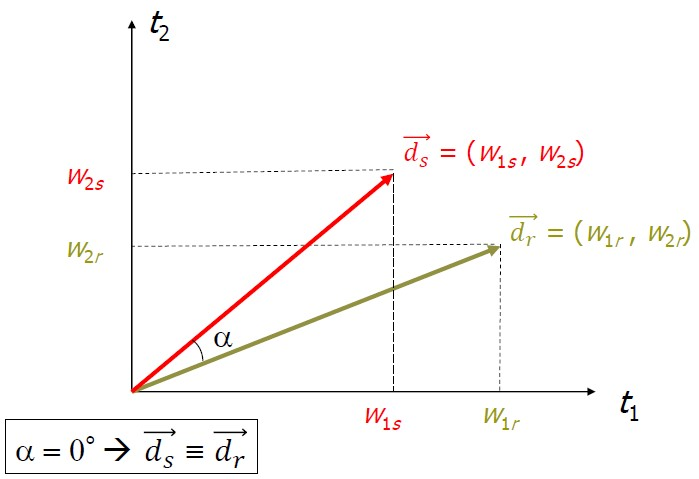
\includegraphics[scale=0.35]{../images/01_5_modello_vettoriale}
	\caption[Rappresentazione di due documenti nello spazio vettoriale]{Rappresentazione di due documenti nello spazio vettoriale}
	\label{fig:vectmodel}
\end{figure}

In questo modo è possibile specificare, per ogni termine che appartiene a un documento, un peso arbitrario positivo che non sia necessariamente binario, per consentire al sistema di tenere in considerazione le frequenze di ogni termine nel documento e nella collezione.

\vspace{1em}

La pesatura dei termini migliora la qualità del risultato è il confronto parziale fra vettori consente di reperire anche documenti che approssimino le condizioni della query senza soddisfarle completamente, garantendo la visualizzazione dei risultati in ordine decrescente di similarità, e quindi di rilevanza.

I limiti principali di questo modello consistono nel fatto che l’assunzione di indipendenza fra i termini è priva di fondamento e che il linguaggio di interrogazione si rivela decisamente poco intuitivo ed espressivo. Per sopperire alle mancanze del linguaggio è possibile combinare i modelli booleano e quello vettoriale affinché il primo si occupi di reperire i documenti rilevanti e il secondo abbia il solo compito di ordinarli, pur sapendo che in questo modo si perde la componente di parzialità sul confronto fra query e documenti. Per operazioni di \textit{matching} più complesse e complete è necessario approcciare modelli matematici più avanzati.



\section{Valutazione di un sistema IR}
\label{sec:IRSrating}

 “L’Information Retrieval è una disciplina che deve cercare di soddisfare \textbf{necessità informative espresse in modo vago e impreciso}, mediante le ambiguità del linguaggio naturale, e deve \textbf{confrontarle in modo approssimativo con le informazioni contenute in un documento}, espresse mediante il medesimo linguaggio naturale.”
\newline [Alan Smeaton, 1997]
% SI METTONO DIVERSAMENTE LE CITAZIONI?

\vspace{1em}

In funzione dei fattori di incertezza con i quali un IRS è tenuto ad operare, si può facilmente dedurre che non sia affatto facile appurare l'affidabilità dei risultati prodotti dal sistema a seguito di una ricerca. Risulta infatti piuttosto complicato riuscire a discriminare se un documento reperito sia effettivamente utile per le esigenze informative dell’utente o se rappresenti invece un elemento di poco conto. 

\vspace{1em}

Il concetto di rilevanza è fondamentale per misurare l’efficacia di un sistema di Information Retrieval. Tale misura è principalmente soggetta a due valutazioni:

\begin{itemize}
\item \textbf{Precisione} (precision), la percentuale di documenti reperiti che risultano effettivamente rilevanti per una certa query, rispetto alla totalità dei documenti reperiti come risultato della query stessa.
\item \textbf{Richiamo} (recall), la percentuale di documenti rilevanti che vengono effettivamente reperiti in seguito a una query, rispetto a tutti quelli rilevanti (per tale query) presenti nella collezione. 
\end{itemize}

\[ Precisione = \frac{|Rilevanti \cap Reperiti|}{|Reperiti|} \]
\[ Richiamo = \frac{|Rilevanti \cap Reperiti|}{|Rilevanti|} \]

\vspace{1em}

È immediato notare che precisione e richiamo siano proprietà effettivamente valutabili solo a patto che si conosca a priori quali sono i documenti a propria disposizione, ed in particolare quali sono quelli rilevanti rispetto alla query che si sta cercando di valutare. Tale valutazione è altamente soggettiva e influenzata anche dall’ambiguità delle richieste sottoposte al sistema dall’utente. Un ulteriore elemento che influisce su questo tipo di valutazione può essere l’incompletezza nella rappresentazione dei documenti, che potrebbe rivelarsi poco adatta per rispondere ad alcune specifiche esigenze.

\vspace{2em}

Oltre alla valutazione d’efficacia, che si basa principalmente sulla bontà della rappresentazione formale dell’archivio e dell’algoritmo di matching utilizzato, un IRS è soggetto ad ulteriori criteri di valutazione più facilmente misurabili:
\begin{itemize}
\item Interazione con il sistema, cioè quali sono le \textbf{funzionalità} che mette disposizione dell’utente e il livello di facilità ed \textbf{intuitività} con le quali siano utilizzabili. 
\item Efficienza, cioè i \textbf{tempi} di risposta alle richieste dell’utente e lo \textbf{spazio} occupato dagli indici su disco.
\end{itemize}

Sulla base di quanto detto, emerge chiaramente che la valutazione di un sistema di reperimento delle informazioni sia un compito molto complesso che richiede un certo livello di esperienza.





